\documentclass[oneside,11pt,openright]{report}
\usepackage[latin1]{inputenc}
\usepackage{listings}
\usepackage[american]{babel}
\usepackage{a4}
\usepackage{latexsym}
\usepackage{amssymb}
\usepackage{amsmath}
\usepackage{amsthm}
\usepackage{epsfig}
\usepackage[T1]{fontenc}
\usepackage{lmodern}
\usepackage[labeled]{multibib}
\usepackage{color}
\usepackage{datetime}
\usepackage{epstopdf} 
\usepackage{graphicx}
\usepackage{pgfplots}
\usepackage[format=hang]{caption}
\usepackage{float}


\lstset{
  frame=none,
  xleftmargin=2pt,
  stepnumber=1,
  numbers=none,
  numbersep=5pt,
  numberstyle=\ttfamily\tiny\color[gray]{0.3},
  belowcaptionskip=\bigskipamount,
  captionpos=b,
  escapeinside={*'}{'*},
  language=haskell,
  tabsize=2,
  emphstyle={\bf},
  commentstyle=\it,
  stringstyle=\mdseries\rmfamily,
  showspaces=false,
  keywordstyle=\bfseries\rmfamily,
  columns=flexible,
  basicstyle=\small\sffamily,
  showstringspaces=false,
  morecomment=[l]\%,
}

\usepackage{pgf,tikz}
\usepackage{comment}
\usetikzlibrary{arrows,automata}
\usetikzlibrary{backgrounds,fit}
\usetikzlibrary{shapes,patterns}
\usetikzlibrary{calc,chains,positioning}

\renewcommand*\ttdefault{txtt}
\newcommand{\BigO}[1]{\ensuremath{\operatorname{O}\left(#1\right)}}
\newcommand{\BigT}[1]{\ensuremath{\Theta\left(#1\right)}}
\newcommand{\specialcell}[2][c]{%
  \begin{tabular}[#1]{@{}c@{}}#2\end{tabular}}
% see http://imf.au.dk/system/latex/bog/

\newcommand{\adjustimg}{% Horizontal adjustment of image
  \ifodd\value{page}\hspace*{\dimexpr\evensidemargin-\oddsidemargin}\else\hspace*{-\dimexpr\evensidemargin-\oddsidemargin}\fi%
}
\newcommand{\centerimg}[2][width=\textwidth]{% Center an image
  \makebox[\textwidth]{\adjustimg\inputgraphics[#1]{#2}}%
}
\newcommand{\NULL}{\textbf{null}}
\newcommand{\cons}{\textbf{cons}}
\newcommand{\cdr}{\textbf{cdr}}

\newcommand{\MakeList}{\textsc{makeList}(x)}
\newcommand{\Push}{\textsc{push}(x,L)}
\newcommand{\Pop}{\textsc{pop}(L)}
\newcommand{\Lookup}{\textsc{Lookup}(d)}
\newcommand{\Inject}{\textsc{inject}(x,L)}
\newcommand{\Eject}{\textsc{eject}(L)}
\newcommand{\Catenate}{\textsc{catenate}(K,L)}

\newcommand{\List}{\textsc{List}}
\newcommand{\PairsLazy}{\textsc{Pairs-Lazy}}
\newcommand{\PairsStrict}{\textsc{Pairs-Strict}}
\newcommand{\RotationLazy}{\textsc{Rotation-Lazy}}
\newcommand{\RotationStrict}{\textsc{Rotation-Strict}}
\newcommand{\HoodMelville}{\textsc{Hood-Melville}}

\newtheorem{prop}{Property}
\newtheorem{theorem}{Theorem}

\begin{document}

%%%%%%%%%%%%%%%%%%%%%%%%%%%%%%%%%%%%%%%%%%%%%%%%%%%%%%%%%%%%%%%%%%%%%%%

\pagestyle{empty} 
\pagenumbering{roman} 
\vspace*{\fill}\noindent{\rule{\linewidth}{1mm}\\[4ex]
{\Huge\sf Functional Queues}\\[4ex]
{\huge\sf Kristoffer Just Andersen, 20051234\\[2ex]
\huge\sf Troels Leth Jensen, 20051234 \\[2ex]
\huge\sf Morten Krogh-Jespersen, 20022362}\\[2ex]
\noindent\rule{\linewidth}{1mm}\\[4ex]
\noindent{\Large\sf Project 3, Advanced Data Structures 2013, Computer Science\\[1ex] 
\monthname\ \the\year  \\[1ex] Advisor: Gerth St�lting Brodal\\[15ex]}\\[\fill]}
\epsfig{file=logo.eps}\clearpage

%%%%%%%%%%%%%%%%%%%%%%%%%%%%%%%%%%%%%%%%%%%%%%%%%%%%%%%%%%%%%%%%%%%%%%%

\tableofcontents
\pagenumbering{arabic}
\setcounter{secnumdepth}{2}

%%%%%%%%%%%%%%%%%%%%%%%%%%%%%%%%%%%%%%%%%%%%%%%%%%%%%%%%%%%%%%%%%%%%%%%

\chapter{Introduction}

This is the third and final report in the Advanced Data Structures
course at Aarhus University and we will in this project investigate
the performance of queues in the functional language by the name of
Haskell.

We first present some terminology and then a total of five different
queues where two only differs by one being lazy. Hereafter, we
describe how we made the implementation and tested for correctness and
why we can say that our implementations are correct.

We then describe how we measure running times in a lazily evaluated
language and explain the different tests we have chosen for testing
the running times of each queue.

Finally, we will give an answer to the problem from the theoretic
project of how to implement a data structure having push and pop in
$\BigO{1}$ while also having index lookup in $\BigO{\log n}$ and
conclude on the entire project.

\section{Terminology}

We will use some specific phrases to describe properties that we,
for good measure, include below:

\paragraph{Purely functional}
Purely functional is a term that is used to describe data structures
where no operation perform destructive updates. Such a data structure
is said to be immutable or persistent. Notice that, in this course, we
further divide persistence into partial persistence and full
persistence, where this is considered to be full persistence.

\paragraph{Strict evaluation}
Strict evaluation (eager evaluation) is where an expression is
computed at the point where it is assigned to a variable or is passed
as an argument.

\paragraph{Lazy evaluation}
Lazy evaluation delays the computation of a variable such that the
expression is computed at the point where the variable is used.

\paragraph{Memoization}
When an expression is bound to a variable, that variable can be used
multiple times. With a strict evaluation, the variable is assigned a
specific value. If a lazy evaluation strategy is used then the first
time the value of a variable is needed, the computation will occur,
but what about subsequent uses? Memoization says that when a value has
been calculated once, that value will be stored and subsequent uses
will therefore not repeat any calculations. The combination of lazy
evaluation with memoization is also called call-by-need.

\chapter{A purely functional list as a queue}

\begin{center}
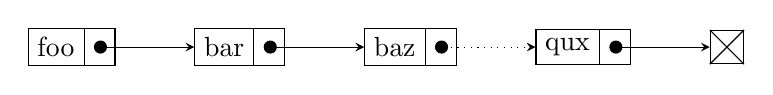
\begin{tikzpicture}
    [list/.style={rectangle split, rectangle split parts=2,
    draw, rectangle split horizontal}, >=stealth, start chain,
    pointer/.style = {font=\tt, anchor=base, inner sep=2pt}]

  \node[list,on chain] (A) {foo};
  \node[list,on chain] (B) {bar};
  \node[list,on chain] (C) {baz};
  \node[list,on chain] (D) {qux};
  \node[on chain,draw,inner sep=6pt] (E) {};

  \draw (E.north east) -- (E.south west);
  \draw (E.north west) -- (E.south east);
  \draw[*->] let \p1 = (A.two), \p2 = (A.center) in (\x1,\y2) -- (B);
  \draw[*->] let \p1 = (B.two), \p2 = (B.center) in (\x1,\y2) -- (C);
  \draw[dotted,*->] let \p1 = (C.two), \p2 = (C.center) in (\x1,\y2) -- (D);
  \draw[*->] let \p1 = (D.two), \p2 = (D.center) in (\x1,\y2) -- (E);

\end{tikzpicture}
\captionof{figure}{A purely functional list}
\label{fig:list_figure}
\end{center}

Figure \ref{fig:list_figure} shows a graphically representation of a
functional list where elements can be inserted at the front by means
of $\cons$ and the list can be traversed by following the arrows which
corresponds to the $\cdr$ operation. The list can be constructed in
constant time by a special termination construction (inductive base
case) being the empty list.

Elements can be inserted and removed from the front in constant time,
but all other operations require traversing the entire list. Below is
all operations with the corresponding time-complexities shown:

\begin{center}
  \begin{tabular}{ l | c | c}
    Operation & List \\ \hline
    \MakeList & $\BigO{1}$ \\ 
    \Push & $\BigO{1}$ \\ 
    \Pop & $\BigO{1}$ \\ 
    \Inject & $\BigO{n}$ \\ 
    \Eject & $\BigO{n}$ \\ 
  \end{tabular}
\end{center}

Because a queue pops elements from the front and injects elements in
the end, this is not the most efficient queue implementation.

\chapter{Queue by a pair of lists}
A simple observation to make is that if we reverse the list of section
2, $\Inject$ and $\Eject$ will be at the front of the list and will
therefore take $\BigO{1}$ time. however, $\Push$ and $\Pop$ will take
$\BigO{n}$ time. A trick is therefore to maintain a pair of lists such
that $\Push$, $\Pop$, $\Inject$ and $\Eject$ for the most part perform
in constant time.

\begin{center}
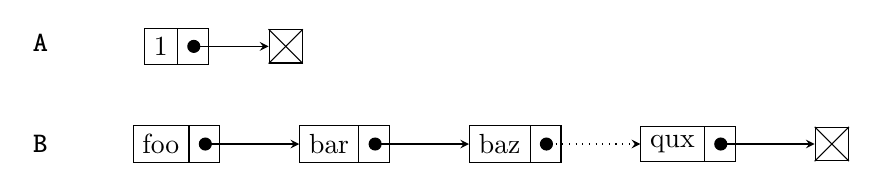
\begin{tikzpicture}
    [list/.style={rectangle split, rectangle split parts=2,
    draw, rectangle split horizontal}, >=stealth, start chain,
    desc/.style = {font=\tt, anchor=base, inner sep=2pt}]

  \node[desc, on chain] (list_b) {B};
  \node[list,on chain] (A) {foo};
  \node[list,on chain] (B) {bar};
  \node[list,on chain] (C) {baz};
  \node[list,on chain] (D) {qux};
  \node[on chain,draw,inner sep=6pt] (E) {};

  \node[desc, above=6ex of list_b] (list_a) {A};
  \node[list, above=5ex of A] (F) {1};
  \node[right=5ex of F,draw,inner sep=6pt] (G) {};

  \draw (G.north east) -- (G.south west);
  \draw (G.north west) -- (G.south east);
  \draw[*->] let \p1 = (F.two), \p2 = (F.center) in (\x1,\y2) -- (G);

  \draw (E.north east) -- (E.south west);
  \draw (E.north west) -- (E.south east);
  \draw[*->] let \p1 = (A.two), \p2 = (A.center) in (\x1,\y2) -- (B);
  \draw[*->] let \p1 = (B.two), \p2 = (B.center) in (\x1,\y2) -- (C);
  \draw[dotted,*->] let \p1 = (C.two), \p2 = (C.center) in (\x1,\y2) -- (D);
  \draw[*->] let \p1 = (D.two), \p2 = (D.center) in (\x1,\y2) -- (E);

\end{tikzpicture}
\captionof{figure}{Maintaining two lists - reverse B and place as A on next pop from A}
\label{fig:two_lists_before_reverse}
\end{center}

When we enqueue nodes they are pushed to the front of list B, and when
elements are removed they are taken from the front of list A. Both of
these operations will normally take constant time. The only problem is
what to do if A is empty.

Figure \ref{fig:two_lists_before_reverse} shows a configuration of the
queue where a pop will result in A becoming the empty list. Subsequent
pops should remove from the end of B but that would take $\BigO{n}$
for every operation. It therefore makes more sense to reverse the list
once and place it instead of A.

To analyze the running time we will use amortization and specifically
use the Potential method \cite[p. 459]{ITA09}. We will use the length
of the the tail list as the potential function. Every insert into tail
is therefore an operation that takes a single step and increases the
potential by one, so the amortized cost is two.

Reversing the list can be done in $\BigO{|tail|}$. The length of the
tail is the number of enqueues since the last reversal or construction
of the list. Therefore, we must have $|tail|$ unreleased potential,
giving us that the tail list can be reversed in $\BigO{1}$ whenever
needed. The queue will have the following time complexities:

\begin{center}
  \begin{tabular}{ l | c | c}
    Operation & List & Two lists amortized / worst case  \\ \hline
    \MakeList & $\BigO{1}$ & $\BigO{1}$ / $\BigO{1}$ \\ 
    \Pop & $\BigO{1}$ & $\BigO{1}$ / $\BigO{n}$ \\ 
    \Inject & $\BigO{n}$ & $\BigO{1}$ / $\BigO{1}$ \\ 
  \end{tabular}
\end{center}

\section{Converting to strict in Haskell}

Laziness is a feature in Haskell. A queue might perform differently
depending on the choice of evaluation. At the very least, the
expensive operations will be performed at different runtime points in
the program. By placing strictness annotations the right places,
(putting ! in front of the two constituent lists) we tell Haskell to
enforce a strict evaluation of the data structure. That is, a value
representing this type of queue will never contain any \emph{thunks}
or unevaluated values.  Because of the way rotations happen only when
needed, we might not see any differences between lazy or eager
evaluation for this queue. Nevertheless, we will perform tests on both
the lazy and the strict version of this queue. We will delay (are we
then lazy?) the discussion about amortized running times for a lazy
version of this queue to the next chapter.

\chapter{Pair of lists with lazy evaluation}

We were asked to implement a queue with lazy evaluation having
amortized constant time for $\Inject$ and $\Pop$. We already have one
such implementation but it might be fun to have another where rotation
occurs at points in execution where the list reversion can be delayed.

Like other functional queues we have two lists; one representing the
front and another representing the tail. At specific points we will
rotate the elements from the tail onto the head by reversing the tail
list and appending it. In Haskell the append and the reverse function
is lazy, giving us the desired evaluation strategy.

The trick with two lists has already been used in the previous chapter
but we will use another trigger for the lazy implementation. We rotate
whenever the length of the tail list is one greater than the length of
the front list.

\section{Analyzing lazy evaluations}

When we calculated the potential in the previous section we made the
assumption that a queue was used ephemerally. We did not discuss
amortized running times when using the \emph{same} queue multiple
times. Consider a queue that has a lot of potential stored and the
triggering of a reversal of the tail list is imminent. The queue is
persistent, meaning, that performing $\Pop$ on the same queue is
non-destructive. Therefore, the expensive operation can be computed
multiple times if we pass the original queue as argument to different
operations. The released potential can only be used once, thereby
ruining our amortized analysis.

There is no way to avoid this computation in language having
call-by-value or call-by-name without using side effects, but for lazy
evaluations with memoization, which we call call-by-need, the
expensive operation is only carried out once. However, memoization is
a side effect and thus, some of our arguing might be considered a test
of faith.

It is inadequate to do amortized analysis for lazy amortized data
structures by arguing as if they were strict \cite{OKA96}. We divide
the cost of an operation two categories; unshared cost and shared
cost. Unshared cost is the cost the operation takes, with the
assumption that all lazy constructions of the data structure, that will
be used, has been computed. The shared cost of an operation is the
time it would take to execute every suspension created but not
evaluated by the operation. The sum of both is called the complete
cost.

To adjust he Potential function we have to replace the savings
function $\Phi$ (we store potential) with a function $\Psi$
representing the upper bound on accumulated debt. The amortized cost
of an operation will therefore be the complete cost of an operation -
the change in potential. With this change we can calculate the
complete cost of an operation as if it is strict.


\section{Completing the analysis of the lazy queue}

We will analyze the lazy queue with our modified potential function
$\Psi$. As always, it should be the case that we add potential on
inserts and release potential when deleting. We therefore define:
\begin{align*}
  \Psi(Q) = |notreversed(F)| + |R|
\end{align*}

Let us analyze the amortized cost of an $\Inject$ operation and let us
consider the case where no rotation occurs. The operation takes one
step and also have to pay to the potential function, which is a total
cost of 2. The enqueue that creates a rotation also takes one step
when adding and also have to pay the cost of increasing the
potential. When the rotation occurs the potential described by $|R|$
will be released by the same amount that $|notreversed(F)|$ increases
resulting in no additional change in potential. Finally, we have to
remember to pay for initiating the rotation which gives a total of 3.

Analyzing $\Pop$ is straight forward, however there are four
cases. The case where $\Pop$ does not force an unevaluated expression
only has the cost of removing the first element. If $\Pop$ forces a
rotation, the cost is 2 per the argument above. If $\Pop$ evaluates an
unevaluated expression, the operation will take $\BigO{n}$, but the
potential will decrease by the same amount, giving us a total cost
of 2. Finally, if $\Pop$ rotates and forces an unevaluated expression
to be computed, the final cost will be 3.

The above analysis assumes that, when a demand for the first element of
a lazy list not yet reversed, the list is reversed and all subsequent
calls to the list will work in constant time. The latter part assumes
therefore that lazy lists are memoized. We can now present the time
complexities for the lazy algorithm:

\begin{center}
  \begin{tabular}{ l | c | c | c }
    Operation & List & \specialcell{Two lists\\ amortized / worst case} & \specialcell{Lazy\\ amortized / worst case} \\ \hline
    \MakeList & $\BigO{1}$ & $\BigO{1}$ / $\BigO{1}$  & $\BigO{1}$ / $\BigO{1}$ \\ 
    \Pop & $\BigO{1}$ & $\BigO{1}$ / $\BigO{n}$ & $\BigO{1}$ / $\BigO{n}$ \\ 
    \Inject & $\BigO{n}$ & $\BigO{1}$ / $\BigO{1}$  & $\BigO{1}$ / $\BigO{1}$ \\ 
  \end{tabular}
\end{center}

\chapter{$\BigO{1}$ lists with worst case $\BigO{1}$ enqueue and dequeue with strict evaluation}

All of the queues described above have worst case running times
$\BigO{n}$ which is unacceptable in some situations. Thus there exists
a need for real times queues where all operations have worst case
running times $\BigO{1}$. We have chosen to implement the
Hood-Melville real time queue \cite{HOM80}, in the style of
\cite{OKA96}.

There is a few key insights to this algorithm. First, reversing a list
incrementally can be done by having two lists and transferring
elements from one to the other. Second, one can incrementally append
two lists by applying the trick. If one would like to append two
lists $xs$ and $ys$, one can reverse $xs$ to $xs'$ and then reverse
$xs'$ onto $ys$. Additionally, one can reverse $xs$ on to the reverse
of $ys$ by reversing $xs$ and $ys$ in parallel and then continue as
before.

Initially, the queue will have two lists forming the head $H$ and tail
$T$ and two integers describing the length of each. When we decide to
rotate, we use the observation above and do the following:

\begin{enumerate}
\item Reverse $T$ forming the tail of the new resulting head $H'$
\item Reverse $H$ into $H_R$
\item Reverse $H_R$ onto $H'$
\end{enumerate}

One should be able to convince him- or herself that queue order
is preserved after the third step. However, the queue will not remain
constant when performing the rotation (which is a weird phrase in
\cite{HOM80} since the incremental rotation only occurs when changes
occur), but basically, it means that we have to maintain the state of
the current rotation and provide the user the ability to still make
alterations to the queue.

Allowing the user to enqueue elements is easily done by just having a
new tail list. Dequeuing is bit harder because we are currently
reversing the $H$ into $H_R$. The answer is to have two lists: one
being a working copy of the old list and one being the list we are
reversing. This again introduces some maintenance because removing an
element from the working copy somehow has to be synchronized with the
list we are reversing. To correct this, we use a counter that describes
how many valid elements to be copied from $H_R$. A total of six lists
is therefore necessary for this data structure.

The copying (or rotation) should be completed before the first
element is needed. We will rotate elements when the tail list becomes
one longer than the head list. Therefore, rotating elements will take
$m+1$ operations to complete Step 1 and $m$ operations to complete
Step 2 Since these can be done in parallel the total time is
$m+1$. Completing Step 3 will take additional $m$ operations giving a
total of $2m+1$. Therefore $2m + 1$ incremental operations must be
performed in at most $m$ queue operations. By performing the two first
rotation steps starting the rotation process and hereafter perform two
incremental steps for each queue operation we should be on the safe
side. In total this gives $2(m+1) = 2m + 2$ steps, which is greater
than $2m + 1$. We therefore perform constant work for every queue
operation.

\begin{center}
  \begin{tabular}{ l | c | c | c | c }
    Operation & List & \specialcell{Two lists\\ amortized/worst} & \specialcell{Lazy\\ amortized/worst} & \specialcell{Hood\\Melville} \\ \hline
    \MakeList & $\BigO{1}$ & $\BigO{1}$ / $\BigO{1}$  & $\BigO{1}$ / $\BigO{1}$ & $\BigO{1}$ \\ 
    \Pop & $\BigO{1}$ & $\BigO{1}$ / $\BigO{n}$ & $\BigO{1}$ / $\BigO{n}$ & $\BigO{1}$ \\ 
    \Inject & $\BigO{1}$ & $\BigO{1}$ / $\BigO{1}$  & $\BigO{1}$ / $\BigO{1}$ & $\BigO{1}$ \\ 
  \end{tabular}
\end{center}

\chapter{Testing and correctness}

Testing a data structure against a specification is traditionally done
using some permutation of black-box and unit testing, as done in the
previous reports. Implementations in C were tested against
hit-and-miss unit tests at the whim of the programmers, to the extent
that their imagination and endurance permitted.

We can do one better with the levels of abstraction permitted by a
functional language -- in particular the type system of Haskell.

%TODO Insert ref to Hughes & Claessen
We test the implementations by using a concept from operational
semantics known as \emph{observational equivalence}, as detailed by
John Hughes \& Koen Claessen \cite{CLA02}. It uses the idea of an
\emph{evaluation context}, a notion of ``the surrounding program'',
and of \emph{observable results}, the effects visible to the
surrounding program caused by running a particular piece of code. Two
pieces of code are then observationally equivalent if they produce the
same observable result in all evaluation contexts.

We here, like the paper, restrict ourselves to ``queue programs'' --
the subset of Haskell dealing only with our queue interface. While we,
for correctness, should consider all of Haskell as evaluation
contexts, we are interested in the behaviour of our implementations,
and -- as opposed to C -- there is no way to manipulate the state of
the queue without going through the interface. Without pointer
arithmetic, side effects and associated suspects, we can be certain of
the absence inadvertent mutation of the international structure of the
queue.

A queue is an inherently ``stateful'' object, and so is typically
used in an imperative fashion. As such we consider imperative-style
monadic programs of Haskell as the context, which only manipulates the
queue through the interface, as argued above. We define a data type for
representing such contexts:

\begin{lstlisting}
data Action = Inject Int
            | Pop
            | Peak
            | Return (Maybe Int)
\end{lstlisting}

representing an inject, a pop, a peak, and the binding of the result
of a peak, respectively. This last action is needed to argue that
instead of obtaining an element from a queue, if we know that element,
we might as well explicitly write that element in the program
ourselves.

We then define a function ``executing'' an evaluation context on a
given queue, collecting observables as it goes. It reads equationally
as one would expect.

\begin{lstlisting}
perform :: Queue q => q Int -> [Action] -> [Maybe Int]
perform q []     = []
perform q (a:as) =
  case a of
    Inject n -> perform (inject n q) as
    Pop      -> perform (pop q) as
    Peak     -> peak q : perform q as
    Return m -> m : perform q as
\end{lstlisting}

Finally, we define a testable property on queues, that asserts that in
all evaluation contexts (prefixes and suffixes of actions on queues)
we observe the same results from evaluating the queue in that context.

\begin{lstlisting}
equiv :: Queue q => q Int -> [Action] -> [Action] -> Property
equiv q c c' =
  forAll (actions 0) $ \pref ->
  forAll (actions (delta (pref ++ c))) $ \suff ->
  let
    observe x =
      perform q (pref ++ x ++ suff)
  in
   observe c == observe c'
\end{lstlisting}

Finally, we wire the property into the QuickCheck library \cite{CLA00}
which generates random evaluation contexts, and verifies 5 assertions
on queues, which according to Hughes \& Claeseen \cite{CLA02} defines
a suitable specification of queues:

\begin{lstlisting}
prop_PeakInject q m n =
  equiv q [Inject m, Inject n, Peak] [Inject m, Peak, Inject n]
prop_InjectPop q m n =
  equiv q [Inject m, Inject n, Pop] [Inject m, Pop, Inject n]
prop_PeakEmpty q =
  equivFromEmpty q [Peak] [Return Nothing]

prop_PeakInjectEmpty q m =
  equivFromEmpty q [Inject m, Peak] [Inject m, Return (Just m)]
prop_InjectPopEmpty q m =
  equivFromEmpty q [Inject m, Pop] []
\end{lstlisting}

The essence of the argument for the specification is to ``bubble''
peeks and pops towards the beginning of the program with the first 3
properties, and then eliminate them with the 2 following properties,
thus ``normalizing'' programs on queues.

Finally we run the test for each of our 4 implementations, creating a
hundred programs of an average length of 8 for each property for a
total of $4 \cdot 5 \cdot 100 = 2000$ unit tests. These are just
default settings and as good as any, but more tests naturally
strengthen the claim that the implementations meet the specifications.

\begin{lstlisting}
runTests :: IO ()
runTests = do test "SimpleQueue" (empty :: BasicQueue Int)
              test "SmartListQueue" (empty :: PairQueue Int)
              test "OkasakiQueue" (empty :: OkasakiQueue Int)
              test "RealTimeQueue" (empty :: RealTimeQueue Int)
  where
    test s q = do putStrLn $ "### Testing " ++ s ++ " ###"
                  suite q
\end{lstlisting}

It is unfortunate that the tests do not conclusively prove the
correctness of our implementations. If only there was a way...

It turns out, there is! As all our data structures are purely
functional and do not use general recursion in the operations, we can
implement the data structures in the Proof Assistant Coq. Which we
did. Coq allows us to state properties on functional programs,
\emph{conclusively prove them}, and then extract the functional
programs to e.g. Haskell. As an added benefit, just by virtue of using
Coq as an implementation we certify our functions total and
terminating, as Coq does not accept partially defined functions.

We start by giving an abstract module declaration of a queue
implementaion.

\begin{lstlisting}
Module Type QUEUE.
  Parameter Q       :           Type -> Type. 
  Parameter inv     : forall A, Q A -> Prop.
  Parameter empty   : forall A, Q A.
  Parameter inject  : forall A, A   -> Q A -> Q A.
  Parameter pop     : forall A, Q A -> Q A.
  Parameter peak    : forall A, Q A -> option A.  
  Parameter to_list : forall A, Q A -> list A.
\end{lstlisting}

The \lstinline{inv} field is a predicate on a queue representing
whatever invariants might be applicable for a given implementation,
and the \lstinline{to_list} function is used to convert a queue to an
ordered list of elements, which we shall use as our model for
specifying queues. Using an abstract model (ordered lists) and then
showing our expectations in the model are satisfied by the
implementation is much in the spirit of observational equivalence: if
looks like we expect in all ways we can measure it, it must be the
same.

Next, we define a series of proof obligations, to describe what must
be proven about a given implementation. Among them are that the
invariant is satisfied by an empty queue, and preserved by all
operations. Do not be alarmed by the use of ``Axiom'': it means ``to
be proven'', not ``to be assumed''.

\begin{lstlisting}
  Definition represents {A : Type} (q : Q A) (l : list A) : Prop :=
    to_list _ q = l.

  Axiom empty_inv :
    forall A, 
      inv A (empty A).

  Axiom inject_inv :
    forall A q x,
      inv A q ->
      inv _ (inject _ x q).

  Axiom pop_inv :
    forall A q,
      inv A q ->
      inv _ (pop _ q).
\end{lstlisting}

The \lstinline{represents} field is used to tie a given instance of a
queue to its representation in the model. With that we can define the
following proof obligations:

\begin{lstlisting}
  Axiom empty_is_empty : forall A,
    represents (empty A) nil.
\end{lstlisting}

The above dictates that an empty queue represents the empty list of
elements.

\begin{lstlisting}  
  Axiom inject_spec :
    forall A l q x,
      represents q l ->
      inv _ q ->
      represents (inject A x q) (l ++ (x :: nil)).
\end{lstlisting}

The above states that injecting an element corresponds to postpending
an element to the ordered list.

\begin{lstlisting}  
  Axiom pop_empty :
    forall A q,
      represents q nil ->
      inv _ q ->
      represents (pop A q) nil.
\end{lstlisting}

The above states that that popping the empty queue returns the empty
queue.

\begin{lstlisting}  
  Axiom pop_xs :
    forall A q x xs,
      represents q (x::xs) ->
      inv _ q ->
      represents (pop A q) xs.
\end{lstlisting}

The above states that popping an element from a queue which represents
the list starting with \lstinline{x} followed by \lstinline{xs} yields
a queue representing \lstinline{xs}.

\begin{lstlisting}    
  Axiom peak_empty_spec :
    forall A q,
      represents q nil ->
      inv _ q -> 
      peak A q = None.
\end{lstlisting}

The above states that peeking an element from an empty queue yields nothing.

\begin{lstlisting}  
  Axiom peak_spec :
    forall A q x xs,
      represents q (x::xs) ->
      inv _ q ->
      peak A q = Some x.

End QUEUE.
\end{lstlisting}

Finally, we state that peeking from a queue representing the ordered
sequence starting with \lstinline{x} yields that \lstinline{x}.

The basic, naive functional queue is an implementation of our model,
and it follows by construction that the proofs are largely
uninteresting. So are the naive implementation based on a pair of
queues. We wont give a detailed account of the proofs of each
implementation, as the proof scripts are quite monstrous to present in
writing. We refer curious readers to \lstinline{Queue.v} in the
accompanying code.

Finally, when all proof obligations are satisfied we run
e.g.
\begin{lstlisting}
Extraction "PairQueue.hs" PairQueue
\end{lstlisting}
to generate a Haskell file with the definitions given in the
module. While slightly unidiomatic in style, the generated code is
exactly as we would have handwritten, and so suffer no performance
penalties.

The generated files are exactly those used in our benchmarks and the
previously outlined random testing, so it is no surprise it satisfied
the previous specification!

We might remark that Coq is a strict programming language which we use
to reason about programs to be run in a lazy setting. This is
inherently not a problem as none of the implementations exploit lazy
capabilities of lazy evaluation but use it only to argue performance
characteristics. We have just proven they have the desired semantics
and so will behave the same in a lazy setting, with the added benefit
of ``lazy performance''.

At the time of writing, we have not succeeded in proving the
Hood-Melville real-time queue correct. Instead, we have made headway
in establishing a usefull invariant by proving that \lstinline{inject}
preserves the empty invariant, and the the empty queue establishes it
-- all under the assumption that it is the right invariant, of
course. Coq still allows extraction to Haskell, however, with loud
warnings about running uncertified code. We believe it doable with
more time and effort invested.

\chapter{Time measurements}

We have a total of five queues - three stricts and two lazy. We are
asked to design benchmarks where a queue is only used once and also
where the queue can be used arbitrarily. In this chapter we explain
how we ensure lazy constructs are evaluated when testing, we describe
the different tests that we apply to the queues and we discuss the
results of said tests.

\section{Making sure that lazy evaluations gets evaluated}

\section{One punch tests}

In this chapter we define only the tests that uses queues ..

We have designed two tests that enable us to directly measure tiem of
insertions and deletions. However, a queue is useful for more things
than theoretic time analysis so we are also using the queue to do
Breadth-First search in graphs.

\subsection{Time of insert}

This tests is analogue to the insert test we performed in Project 2. We would like to investigate, on average, how long it takes for a number of insertions to be inserted depending on the size of the queue. We fill up the queue to some amount $x$ and then perform a constant number of inserts. The total time is then divided by the constant and we have a measure for how long a single insert takes depending on the size of the queue.

\subsection{Time of delete}

This test is almost the same as testing time of insert, except that we delete a constant number of elements. The total time is then again divided by the constant and a measure for how long da single delete takes.

\subsection{Breadth-First Search}

A classic application of queues in functional programming is in a
breadth first traversal of a tree. We made a test case that traversed
a complete balanced binary tree of increasing depths. The case
exercises the queue with an even mix of injects and pops, where every
element is enqueued and popped exactly once for a total of $2^d$ of
each operations for a tree of depth $d$.

\section{Rocky tests (multiple punches - movie reference)}

In this section we describe tests that perform more than one operation
on the same queue. These experiments are necessary because of the
persistent nature of queues and for a more in depth discussion see
sectionXX.

\subsection{Insert onto the same queue}

 This test is designed to hit worst cases on all our queue
implementations, if hitting such a thing is possible. As in the single
usage case, we fill the queue up to some length $n$. Herefter, we
delete insert c times on the queue given as argument, then insert c on
the queue given as argument, insert an element such that the size is
$n+1$ and do the same thing over again. We stop when we have performed
the $2 \cdot n$ iterations.

\subsection{Merge sort}

We define a version of merge-sort in terms of queues. Given $c$ queues
of size $n$, where c i a constant and where elements are ordered by
apperance in the queue, merge all elements into a single queue.

The elements of the queue is generated at random with numbers between
the last element inserted in a list $q$ and $|q| \times M/n$.

For each iteration, a fold is applied to the list of queues where the
accumulating information is the currently smallest element, the tail
of the queue the pop was performed on and the index of the q in the
list. The result is stored in a local variable. Hereafter, a map is
performed on the same list, where all queues are passed along, except
the one that had the smallest element, which is replaced by the tail
of the previous queue. The mapped result is then given as argument to
the next iteration.

Performed on different initial lengths of the queues, we hope to see a
number of expensive operations performed multiple times on the same
queue.

\section{Results}

\subsection{Time of insert}

\subsection{Time of delete}

\subsection{Results of Breadth-First Search}

Below is the graph-plot of the Breadth-First Search results. (Maybe logarithmic x-scale?)

\input{results_BST_nolist}

Comparing the lazy evalution results we can see that $\RotationLazy$ performs worse than $\PairsLazy$, which almost performs almost the same as $\HoodMelville$. The reason has something to do with the amount of rotations that is performed. For $\PairsLazy$ there is exactly one rotation per level, giving us 15 in total, which is easy to see because when a level is completed, the tail list will contain all childs for the next level and the head list will be empty. 

For $\RotationLazy$, there will be two rotations for each level. We will give a simple argument. In the very best case, beginning on a new level, all elements $n$ will be in the head list $H$. This is the farthest from a rotation we can be. Since every dequeue will add two new elements to the tail a rotation will occur in the $n/2$ step when adding the left child to the queue. After rotation and the completed $n/2$ steps,we have $|H| = n - n/2 + n - 1 = 3/2n-1$ and $|T| = 1$, with the remaining $n/2$ nodes of the level yet to be dequeued. After $n/2$ dequeues the $|H|=n-1$ if no rotation happens but the tail would be $|T|=n+1$ and another rotation would therefore have happened. There is no way of avoiding at least two rotations per level.

\section{Rocky tests (multiple punches - movie reference)}

\subsection{Insert onto the same queue}

\input{results_WorstCase_nolist}

\subsection{Merge sort}

\begin{minipage}[c]{\textwidth}
\advance\leftskip-2.5cm
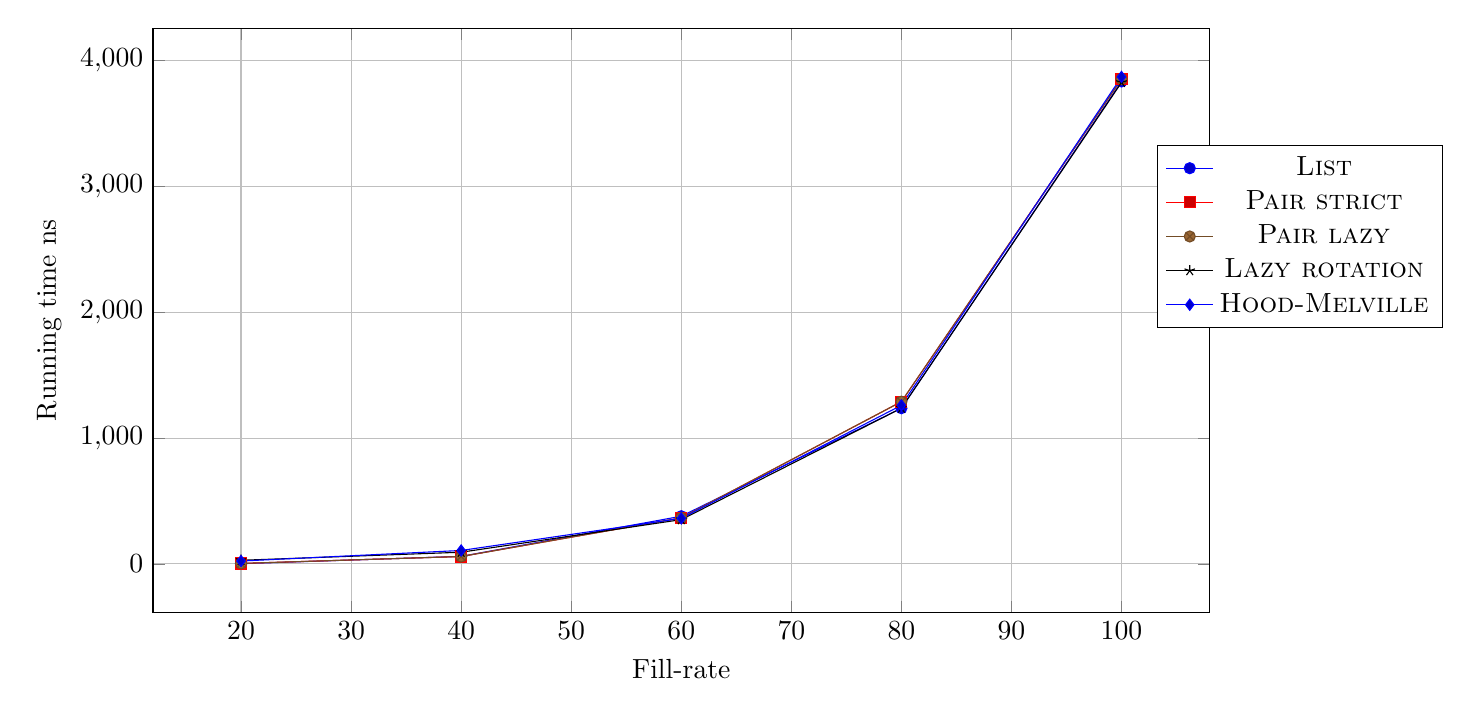
\begin{tikzpicture}
        \begin{axis}[
            xlabel = Fill-rate,
            ylabel = Running time ns,
            height=9cm,
            width=15cm,
            grid=major,
            legend style={
            at={(0.95,0.8)},
            anchor=north west}]            
            legend pos=center west
    	]
    		
    		
    	\addplot coordinates {
(20,2)
(40,60)
(60,379)
(80,1237)
(100,3833)

    	};
        
    	\addlegendentry{\textsc{List}}

                \addplot coordinates {
(20,4)
(40,59)
(60,366)
(80,1289)
(100,3852)

    	};
        
    	\addlegendentry{\textsc{Pair strict}}

        \addplot coordinates {
(20,4)
(40,59)
(60,366)
(80,1289)
(100,3852)

    	};
        
    	\addlegendentry{\textsc{Pair lazy}}

        \addplot coordinates {
(20,29)
(40,93)
(60,352)
(80,1237)
(100,3825)

    	};
        
    	\addlegendentry{\textsc{Lazy rotation}}

        \addplot coordinates {
(20,23)
(40,107)
(60,362)
(80,1260)
(100,3869)

    	};
        
    	\addlegendentry{\textsc{Hood-Melville}}

        \end{axis}

    \end{tikzpicture}
    \captionof{figure}{TITEL}
    \label{fig:sample_figure}
\end{minipage}

\chapter{Functional lists with index lookup}

This exercise was posted in the theoretical project but solving it
seemed natural considering this project is all about functional data
structures.

We are asked to describe a strict functional data structure supporting
\\ $\Push$, $\Pop$ in $\BigO{1}$ and $\Lookup$ in time $\BigO{\log n}$
where $n$ is the number of elements in the list.

By using a standard list composed by $\cons$ we will have a $\Push$
and $\Pop$ in constant time, so how do we solve lookups in $\BigO{\log
  n}$? A binary tree would give us the desired running times. The
problem is how to combine the two. Okasaki solved this problem by
having a collection of complete binary trees~\cite{OKA96}.

For each entry in our list we store a tuple consisting of a complete
binary tree and the size the tree. Thus, the size of the trees is on
the form $2^k-1$. Whenever two adjacent elements are at the front of
the list and another element is pushed, the trees are joined with the
newly added element as the root which gives us that the elements in
any of the binary trees is stored in preorder. Elements 1 to $\lfloor
n / 2 \rfloor$ will be in the left part of the tree and $\lceil n / 2
\rceil$ to $n-1$ will be in the right part.

\begin{center}
  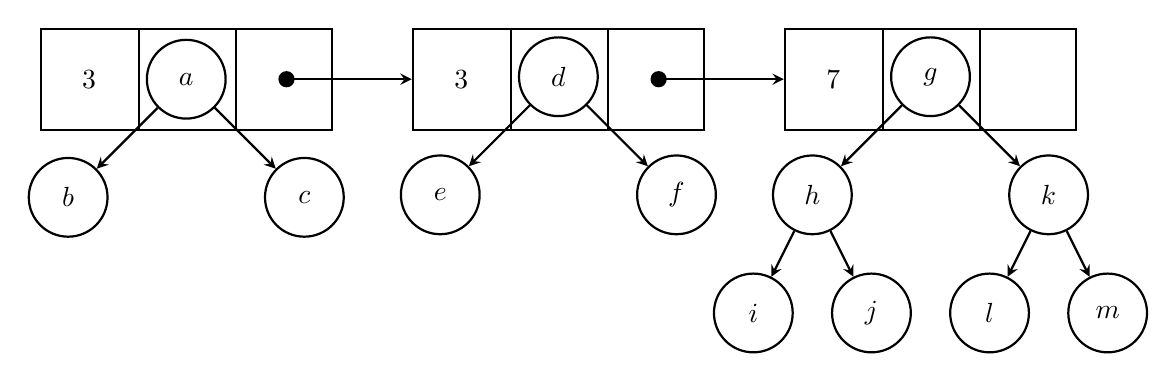
\begin{tikzpicture}[level distance=1.5cm,
  level 1/.style={sibling distance=3cm},
  level 2/.style={sibling distance=1.5cm},
  thick,->,auto,
  list/.style={rectangle split, rectangle split parts=3,
    draw, rectangle split horizontal,minimum size=15pt,inner sep=15pt}, >=stealth, start chain,
    desc/.style = {font=\tt, anchor=base, inner sep=2cm}]
    \tikzstyle{node}=[circle, minimum size=1cm, draw]
    
    \node[list,on chain]    	  (1st) {$3$};
    \node[node]         (a) {$a$}
      child{node[node]    (b) {$b$}}
      child{node[node]    (c) {$c$}};
      
    \node[list,on chain]    	  (2nd) {$3$};
    \node[node,below=-1.2cm of 2nd]         (d) {$d$}
      child{node[node]    (e) {$e$}}
      child{node[node]    (f) {$f$}};

    \node[list,on chain]    	  (3rd) {$7$};
    \node[node,below=-1.2cm of 3rd]         (d) {$g$}
     child{node[node]      (2) {$h$}
      child{node[node]    (4) {$i$}}
      child{node[node]    (5) {$j$}}}
    child{node[node]      (3) {$k$}
      child{node[node]    (6) {$l$}}
      child{node[node]    (7) {$m$}}};

  \draw[*->] let \p1 = (1st.three), \p2 = (1st.center) in (\x1,\y2) -- (2nd);
  \draw[*->] let \p1 = (2nd.three), \p2 = (2nd.center) in (\x1,\y2) -- (3rd);

  \end{tikzpicture}
\captionof{figure}{A list consisting of three complete binary trees, two of size 3 and one of size 7. An added node would result in two complete binary trees of size 7 and an additional node would result in one tree of size 15.}
\label{fig:two_lists_before_reverse}
\end{center}

Inserting new elements can at most join two trees. Since the left
child of the resulting tree will be the first tree in the list and the
right child will be the second tree, the tree can be constructed in
constant time. Similarly, it can be destructed into two parts by just
removing the root and $\cons$ the right child followed by the left
child onto the list.

Looking up and element by index can be done by simply iterating the
list until the containing tree has been found. If the index to search
for is smaller than the size of the tree at the current position said
tree will contain the element, otherwise subtract the size from the
index and continue searching.

If we only have on complete binary tree looking up an element can
clearly be done in $\BigO{\log n}$ time so we have to show that the
length of the list will never be longer than $\log n$.

An integer on the form $2^k-1$ is called a skew-binary term, and if
$t$ is such a term then the next skew-binary term will be $2t+1$. A
decomposition of an integer $n$ greater or equal to zero will be a
multiset of skew-binary terms $\{t_1,t_2,\cdots,t_m\}$ where $n = t_1
+ t_2 + \cdots + t_m$. Such a decomposition is said to be greedy if
the largest term is as large as possible and the remaining part of the
decomposition is greedy as well. In other words a collection of
skew-binary terms is greedy if no subset of lesser terms sums to a
larger term. We will describe such a greedy decomposition of $n$ as
$G(n)$.

\begin{prop}
\label{prop1}
Every integer $n \geq 0$ has a unique greedy decomposition.
\end{prop}
\begin{proof}

$G(0)$ will have the empty set which is unique. For $G(n)$ where
  $n>0$, we know, that no subset of skew-binary terms may sum to a
  larger term thus the it must include the largest possible term $t$
  such that $t \leq n$. We add $t$ to the set and continue searching
  for $G(n-t)$.  Notice, that no subset of $G(n-t)$ can sum to $t$
  otherwise it would not be the largest term respecting $t \leq n$.
\end{proof}

\begin{prop} A skew-binary decomposition is greedy iif every term is unique except \label{prop2}
the two smallest: $t_1 \leq t_2 < t_3 < \cdots < t_m$.
\end{prop}
\begin{proof}
$\\ \Rightarrow$ We have a greedy decomposition and say we have two terms of size $2^k-1$ and a third term of equal or lesser size. Then the three terms would be greater or equal to another term because the next term would be at least as large as $2(2^k-1)+1$. But then this would not be greedy and we have a contradiction.\\
$\Leftarrow$ Again, because the next skew-binary term for any term $t$ is on the form $2t+1$, no two terms can sum up to another term if we only repeat the smallest ones twice and all others are unique. The decomposition would therefore be greedy.
\end{proof}

\begin{theorem} $|G(n)| \leq \lceil \log (n+1) \rceil$.
\label{thm1}
\end{theorem}
\begin{proof}
Clearly if $n=0$ it holds so we turn our attention to $n > 0$. Assume,
to obtain a contradiction, that $|G(n)|$ contains more than $k=\lceil
\log (n+1) \rceil$. Then, by \ref{prop2} and by how a greedy
decomposition is defined, it must be that $G(n)$ contains a term at
least as large as $2^k-1 \geq n$. Then, because $|G(n)|$ contains more
than $k$ terms there is at least one more term and therefore the sum
of terms in $G(n)$ will strictly exceed $n$ and we obtain a
contradiction.
\end{proof}

Except for the two first trees in our list every size of the complete
binary trees in the list is unique and in increasing order by
construction. Therefore, the length of the list can not exceed $\lceil
\log (n+1) \rceil$ by \ref{thm1}. Therefore, lookup will traverse at
most $\BigO{\log n}$ elements in the list and perform a search in a
single complete binary tree of height at most $\log n$.

\chapter{Conclusion}

\addcontentsline{toc}{chapter}{Bibliography}
\bibliographystyle{plain} 
\bibliography{report}

\end{document}
